\chapter{Evaluation}
\label{chap:evaluation}

To evaluate presented map-merging algorithm~\ref{chap:mergingalgorithm} and test performance of implemented map-merging node~\ref{sec:map_merge-package} I used $2$ data sources. First data source was simulation running several P3DX robots. Map-merging node was running through the whole exploring session testing online behaviour of the algorithm. Second data source were maps produced by \gls{SLAM} on \gls{MIT} dataset \#reference here\#. \gls{MIT} dataset produced using a single PR2 robot starting from different locations. Although this data does not come from multi-robot mapping, it is possible to test offline merging performance.

\section{Simulation setup}

I used \gls{VREP} simulator for experiment. All simulated robots were Pioneers P3-DX, which formed a homogeneous exploring team. Robots were setup using \texttt{p3dx\_robot} \# reference here \# package, which also setups \gls{SLAM} and navigation for robots. Robots were using \texttt{hector\_slam} package providing \gls{SLAM} algorithm and \texttt{move\_base} package providing navigation for robots.

Cluster of 5 computers was formed to run simulator, robots, map-merging and exploring nodes. \gls{ROS} network was configured across all workstations using a single \gls{ROS} master running \texttt{roscore}. Every robot was using its own \gls{ROS} namespace for topics and was using a prefix for published \texttt{tf} frames to allow running multiple robots under the same \gls{ROS} master. This setup is well supported in \texttt{p3dx\_robot} package.

While \gls{VREP} is powerful and feature-rich simulator, its usage for multi-robot simulation have some limitations. First of all, \gls{VREP} support for headless mode (running without graphical environment) is not complete. Virtual framebuffer or similar technology is required, which adds performance overhead. Further \gls{VREP} does not scale properly to large number of threads, limiting number of robots for which simulation runs at bearable speed. For this reason it wasn't possible  to test more than 4 robots with this setup.

\section{\gls{MIT} dataset}

\gls{MIT} dataset are data available as rosbags from \#reference here\#. Data comes from mapping multi-floor \gls{MIT} building with PR2 robot. I have used only datasets from the second floor.

For all rosbags I have created maps using the \texttt{hector\_slam} package. It is same \gls{SLAM} algorithm, which was used in simulation. This resulted in $36$ occupancy grid maps with $2048 \times 2048$ cells each.

Produced maps has been statically served in \gls{ROS} with running map-merging node. This setup is therefore limited to test offline merging, but allows a greater number of maps to participate in merging.

It is important to node that presented maps were created by a single robot in multi-session mapping. It is not a result of multi-robot mapping, although the robot initial positions vary between sessions and produced maps are similar to maps we would expect from multi-robot mapping.

\section{Minimal overlapping area}

Presented merging algorithm~\ref{chap:mergingalgorithm} relies on overlapping areas of occupancy grids to produce a merged map. Minimal overlapping area to produce a reliable merge depends on explored environment. Areas with high number of features in occupancy grids require small overlaps and vice versa.

Experiments showed that a reliable merge requires only about $90$ inliers, sometimes only a $80$ inliers is enough to produce a correct transformation as seen in excerpt~\ref{fig:minimal-overlapping-area-log}. This excerpt is from log of map-merging node~\ref{sec:map_merge-package} acquired during simulation. Full log containing number of matches and number of inliers required to produce a transformation along with other details is available in attachments, see section~\ref{chap:files}.

\begin{figure}
    \centering
	\begin{code}
AffineMatcher: have 121 matches
estimate:
[1.002576035215622, 0.00299917716022613, 62.49276756175958;
 -0.00299917716022613, 1.002576035215622, -240.2015971108993]
num_inliers 83
AffineMatcher: have 147 matches
estimate:
[1.002175802299877, -0.0004136975345276905, -15.26120294301828;
 0.0004136975345276905, 1.002175802299877, -120.7595895934327]
num_inliers 95
AffineMatcher: have 193 matches
estimate:
[1.000933706668138, 0.001232315845354937, 78.01218357952351;
 -0.001232315845354937, 1.000933706668138, -119.6792960984003]
num_inliers 157
	\end{code}
    \caption{Excerpt from log of map-merging node captured during simulation. Shows output of matching phase of the algorithm for $3$ pairwise matches along with number of inliers.}
    \label{fig:minimal-overlapping-area-log}
\end{figure}


Simulation featured $3$ robots exploring common area. Figure~\ref{fig:minimal-overlapping-area-scene} show scene used in experiment and initial robots positions.

\begin{figure}
    \centering
    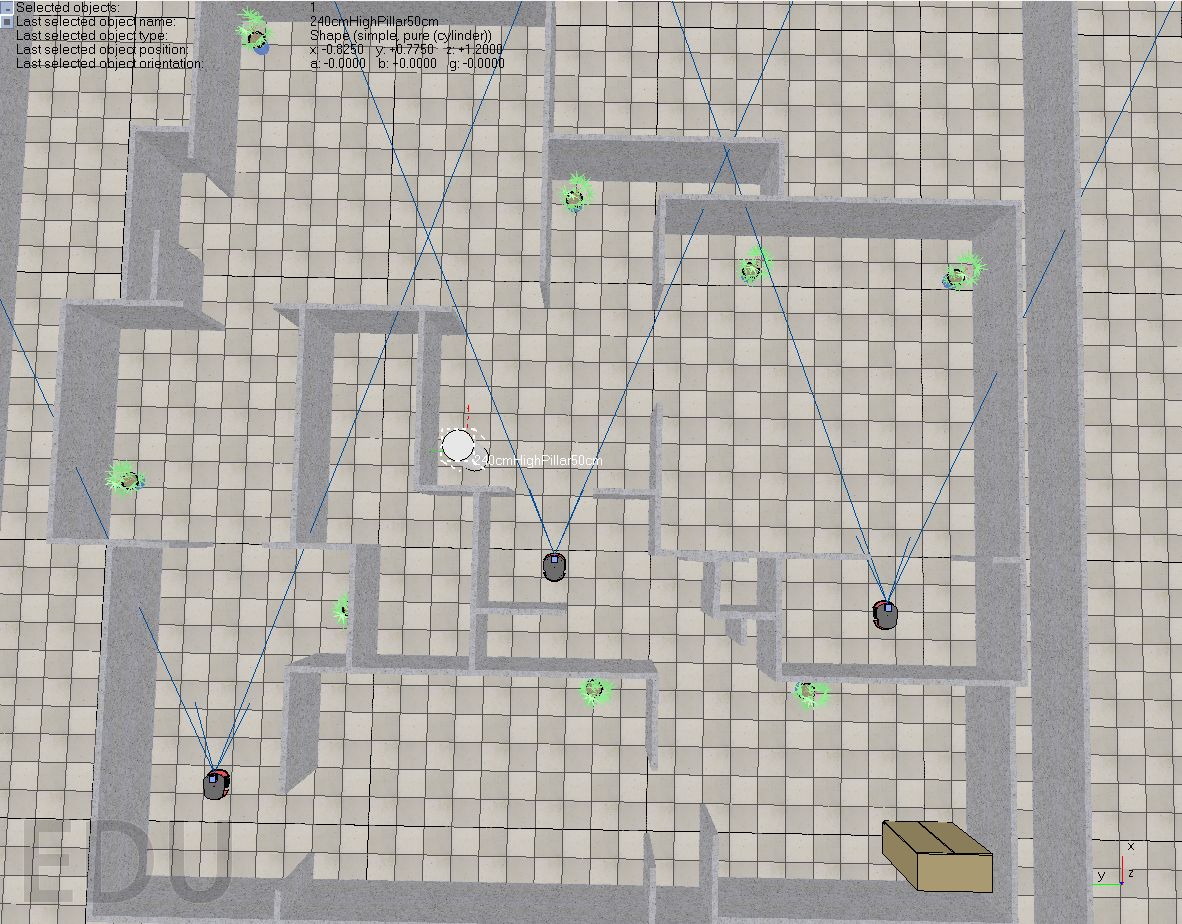
\includegraphics[width=3.93in]{../img/minimal-overlapping-area-scene.png}
    \caption{Scene for experiment with $3$ robots as seen in \gls{VREP} simulator. Robot positions in scene ware used as initial positions of robots for experiment.}
    \label{fig:minimal-overlapping-area-scene}
\end{figure}

\begin{figure}
    \centering
    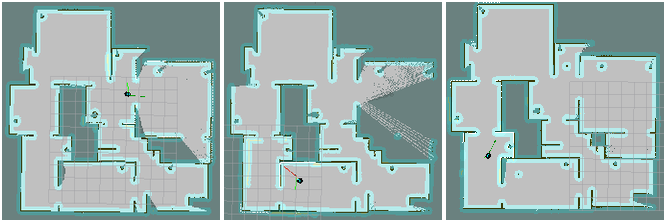
\includegraphics[width=2.22in]{../img/minimal-overlapping-area-final-maps.png}
    \caption{Maps produced by multi-robot mapping in simulator. Simulated scene can be seen in figure~\ref{fig:minimal-overlapping-area-scene}. Robots' positions are final positions when robots finished mapping.}
    \label{fig:minimal-overlapping-area-final-maps}
\end{figure}

\begin{figure}
    \centering
    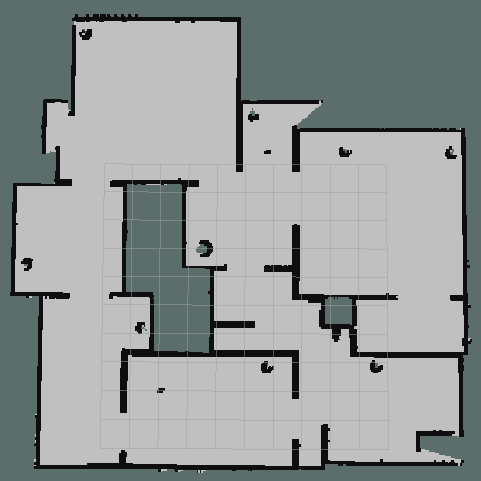
\includegraphics[width=1.58in]{../img/minimal-overlapping-area-merged-map.png}
    \caption{Merged map produced by map-merging node. Map was produced from $3$ maps from figure~\ref{fig:minimal-overlapping-area-final-maps}.}
    \label{fig:minimal-overlapping-area-merged-map}
\end{figure}
